
\chapter{Machine Learning} \label{ML}

\section{introduction}

" We use AI so much that we have stopped thinking of it as AI, ”  says Nello Cristianini,  professor of artificial  intelligence at the University of Bristol.

Nowadays we make a lot of decision based on our past experiences  or our expectations of the future either way we sure tale  a lot of bad decision and make a lot of mistakes , Machines ( computers ) Can be a powerful tool for this kind of tasks with higher prediction ( about future )  and better accuracy , and that is Machine learning which actually a process  that teaches computers to tackle vast amounts of data, pull out patterns, These patterns can represents a model able to  make decisions , But these models are still yet in need of human supervision to evaluate it and help it overcome the complexities Sometimes Hidden in Data .

In this Chapter we will First define Supervised learning and presents One of The powerful Application of such type of learning ( supervised ) SVM Algorithm ( support vector machine )  and Nearest neighbor algorithm , And then Define the second type unsupervised learning   with a review K-means algorithm , these algorithm  proved  to be accurate and robust  for our HGR system as it's going to be shown in  Chapter  [\ref{hgr}]

\section{Supervised Machine Learning}

The majority of practical machine learning uses supervised learning.
Supervised learning is where we have input variables (x) and an output variable (Y) and we use an algorithm to learn the mapping function from the input to the output.

$Y = f(X)$

The goal is to approximate the mapping function so well that when we have new input data (x) that we can predict the output variables (Y) for that data.

It is called supervised learning because the process of an algorithm learning from the training dataset can be thought of as a teacher supervising the learning process.\\ We know the correct answers, the algorithm iteratively makes predictions on the training data and is corrected by the teacher. Learning stops when the algorithm achieves an acceptable level of performance.
Supervised learning problems can be further grouped into regression and classification problems.

\textbf{Classification:} A classification problem is when the output variable is a category, such as “red” or “blue” or “disease” and “no disease”.\\ \textbf{Regression:}  A regression problem is when the output variable is a real value, such as “dollars” or “weight”.
Some common types of problems built on top of classification and regression include recommendation and time series prediction respectively.\\Some popular examples of supervised machine learning algorithms are:\\
Linear regression for regression problems.\\
Support vector machines for classification and regression problems.




\section{Support Vector Machines (SVM) }\label{sec:svm}
As Hill, T., Lewicki, P. Define it in \cite{svm} Support Vector Machines are based on the concept of decision planes that define decision boundaries. A decision plane is one that separates between a set of objects having different class memberships. A schematic example is shown in the illustration below. In this example, the objects belong either to class GREEN or RED. The separating line defines a boundary on the right side of which all objects are GREEN and to the left of which all objects are RED. Any new object (white circle) falling to the right is labeled, i.e., classified, as GREEN (or classified as RED should it fall to the left of the separating line).


\begin{figure}[H]
\centering
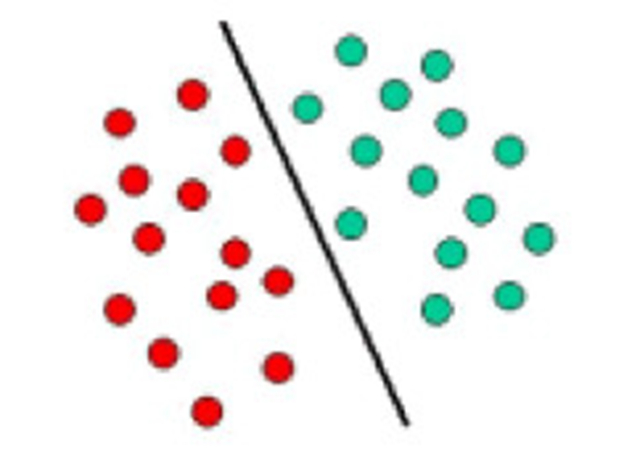
\includegraphics[width=0.3\textwidth]{img/svm1.png}
\caption{example of linear Hyperplan seperating Green data from Red data }
\label{122 }
\end{figure}


The above is a classic example of a linear classifier, i.e., a classifier that separates a set of objects into their respective groups (GREEN and RED in this case) with a line. Most classification tasks, however, are not that simple, and often more complex structures are needed in order to make an optimal separation, i.e., correctly classify new objects (test cases) on the basis of the examples that are available (train cases). This situation is depicted in the illustration below. Compared to the previous schematic, it is clear that a full separation of the GREEN and RED objects would require a curve (which is more complex than a line). Classification tasks based on drawing separating lines to distinguish between objects of different class memberships are known as hyperplane classifiers. Support Vector Machines are particularly suited to handle such tasks


\begin{figure}[H]
\centering
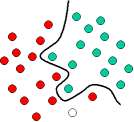
\includegraphics[width=0.3\textwidth]{img/svm2.png}
\caption{Non linear Example of data  }
\label{123 }
\end{figure}

The illustration below shows the basic idea behind Support Vector Machines. Here we see the original objects (left side of the schematic) mapped, i.e., rearranged, using a set of mathematical functions, known as kernels. The process of rearranging the objects is known as mapping (transformation). Note that in this new setting, the mapped objects (right side of the schematic) is linearly separable and, thus, instead of constructing the complex curve (left schematic), all we have to do is to find an optimal line that can separate the GREEN and the RED objects.

\begin{figure}[H]
\centering
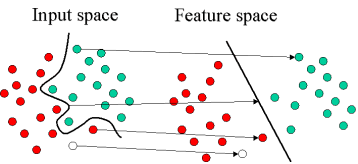
\includegraphics[width=0.5\textwidth]{img/SVMIntro3.png}
\caption{Non linear separated using kernel (higher dimension) }
\label{124 }
\end{figure}


\subsection{Hard-Margin SVM}
The SVM technique is a classifier that finds a hyperplane or a function $g(x) = {\omega}^T +  b$   that correctly separates two classes with a maximum margin.figure below shows a separating hyperplane corresponding to a hard-margin SVM (also called a linear SVM).

\begin{figure}[H]
\centering
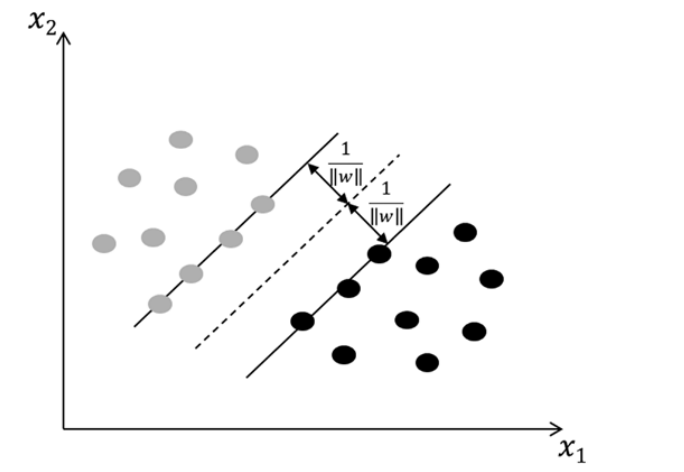
\includegraphics[width=0.5\textwidth]{img/hardmargin.PNG}
\caption{ Hard-maximum-margin separating hyperplane. }
\label{125 }
\end{figure}


\subsection{Soft-Margin SVM}

When the data are not completely separable, as with the points marked by a X in Figure below  , slack variables Xi  are introduced to the SVM objective function to allow error in the misclassification. SVM, in this case, is not searching for the hard margin, which will classify all data flawlessly. Instead, SVM is now a soft margin classifier; that is, SVM is classifying most of the data correctly, while allowing the model to misclassify a few points in the vicinity of the separating boundary

\begin{figure}[H]
\centering
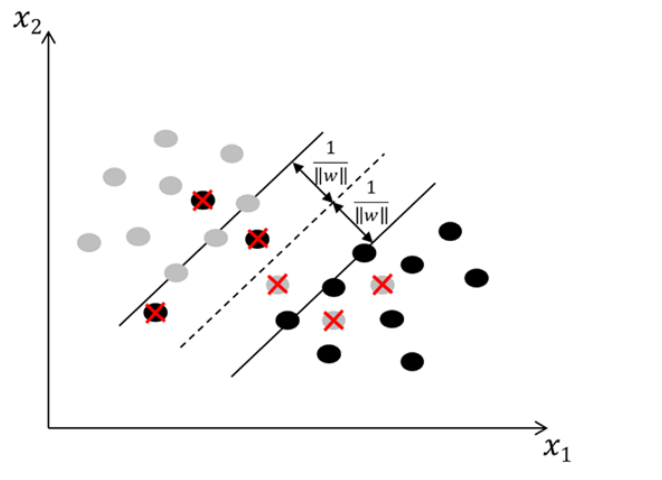
\includegraphics[width=0.5\textwidth]{img/softmargin.PNG}
\caption{  A few misclassifications, as part of soft-margin SVM . }
\label{126 }
\end{figure}


\subsection{Kernels}

When a problem is not linearly separable in input space, soft-margin SVM cannot find a robust separating
hyperplane that minimizes the number of misclassified data points and that generalizes well. For that, a kernel can be used to transform the data to a higher-dimensional space, referred to as kernel space, where data will be linearly separable. In the kernel space a linear hyperplane can thus be obtained to separate the different classes involved in the classification task instead of solving a high-order separating hypersurface in the input space. This is an attractive method, because the overhead on going to kernel space is insignificant compared with learning a nonlinear surface. A kernel should be a Hermitian and positive semidefinite matrix and needs to satisfy Mercer’s theorem, which translates into evaluating the kernel or Gram matrix on all pairs of data points as positive and semidefinite, forming

$K(\small{x,u})=\sum\limits_{r} \phi(x)\phi(u) $ .

where $\phi(x) $ belongs to the Hilbert space.
\newline
$$\int \int K(x,u) g(x) g(u) du dx \geq 0 \ \ \ \ \forall g(x) , \ where \int g^2(x) dx < +\infty$$
\\
\newline 
Some popular kernel functions include


\begin{itemize}

  \item  Linear kernel  : 
  \begin{align*}
  \mathlarger {K(x,u)=  x^{T}.u  }
   \end{align*}
  \item Polynomial function: 
  \begin{align*}
  K(x,u)=(ax^{T}u + c)^{q} ,\, q>0.
  \end{align*}
  \item Gaussian radial basis function (RBF): 
\begin{align*} 
 K(x,u) = e^{\mathlarger{\frac{\mathbf{-\| x -  u\|^2}}{\mathbf{\sigma^2} } }}
\end{align*}
   
  \item  Hyperbolic tangent (sigmoid):
    \begin{equation}
      K(\mathbf x, \mathbf u) = \tanh(\mathbf {\beta} \mathbf x^{T} \mathbf u - \mathbf{\delta})^p
    \end{equation}
    
    \item Laplacian radial basis function : 
    
    \begin{align*} 
      K(x,u) = e^{\mathlarger{\frac{-\| x -  u\|}{\sigma} } }
     \end{align*}
    
\end{itemize}

Kernel selection is heavily dependent on the data specifics. For instance, the linear kernel—the simplest
of all—is useful in large sparse data vectors. However, it ranks behind the polynomial kernel, which avoids
zeroing the Hessian. \\The polynomial kernel is widely used in image processing, The Gaussian and Laplace RBFs are general-purpose kernels
that are mostly applied in the absence of prior knowledge. \\A kernel matrix that ends up being diagonal indicates that the feature space is redundant and that another kernel should be tried after feature reduction.\\

\textbf{
Note} that when kernels are used to transform the feature vectors from input space to kernel space for linearly non-separable datasets, the kernel matrix computation requires massive memory and computational
resources, for big data . 



\section{Nearest Neighbour Based Classifiers}

One of the simplest decision procedures that can be used for classification is the
nearest neighbour (NN) rule. It classifies a sample based on the category of its nearest
neighbour.When large samples are involved,it can be shown that this rule has a
probability of error which is less than twice the optimum error
—hence there is less
than twice the probability of error compared to any other decision rule. The nearest
neighbour based classifiers use some or all the patterns available in the training set
to classify a test pattern. These classifiers essentially involve finding the similarity
between the test pattern and every pattern in the training set.

\subsection{Nearest Neighbour Algorithm}
The nearest neighbour algorithm assigns to a test pattern the class label of its closest
neighbour

% Insert the algorith

\begin{algorithm}[H]
\SetAlgoLined

 initialization\;
 $ A=(X_{1},\omega_{1}),(X_{2},\omega_{2}),....,(X_{n},\omega_{n}) \ // A\ is\ the\ set\ of\ N\ training\ pattern $\\
 
 
$ //where\  X_{i}\ is\ of\ dimension\ n\ and\  \omega_{i}\ is\ the\ class\ label\ of\ the\ i^{th}\ pattern $\\
 
 
 $d(u,x) = \sqrt{\sum_{k=0}^{N} (u_{i}-x_{i})^{2}}  // \ Euclidean\ distance\ measure $\\ 

 \While{ i \neq N }{ // N samples
 
  d(X_{t},X_{i}) = min {D(X_{t},X_{i})}\; 
 
 }
 
 $ X_{t} = \omega_{k} $ \\
 
 $ pattern\ X_{t}\ is\ assigned\ to\ a\ class\ \omega_{k}\ associated\ with\  X_{k} $
 
 \caption{Algorithm for NN}
\end{algorithm}

\vspace{5mm}
\textbf{Example of the algorithm} :\newline 
$ X1 = (0.8, 0.8, 1), X2 = (1.0, 1.0, 1), X3 = (1.2, 0.8, 1)$\\
$X4 = (0.8, 1.2, 1), X5 = (1.2, 1.2, 1), X6 = (4.0, 3.0, 2)$\\
$X7 = (3.8, 2.8, 2), X8 = (4.2, 2.8, 2), X9 = (3.8, 3.2, 2)$\\
$X10 = (4.2, 3.2, 2), X11 = (4.4, 2.8, 2), X12 = (4.4, 3.2, 2)$\\
$X13 = (3.2, 0.4, 3), X14 = (3.2, 0.7, 3), X15 = (3.8, 0.5, 3)$\\
$X16 = (3.5, 1.0, 3), X17 = (4.0, 1.0, 3), X18 = (4.0, 0.7, 3)$


\begin{figure}[H]
\centering
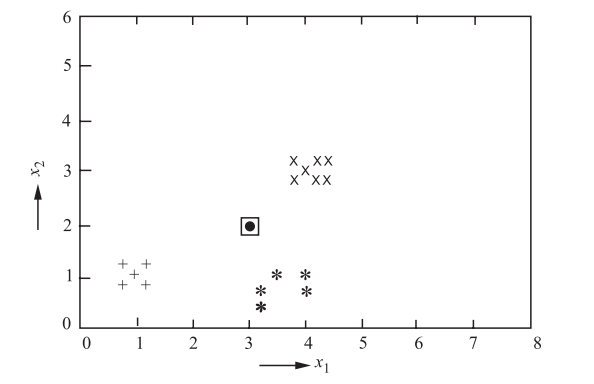
\includegraphics[width=0.6\textwidth]{img/nn-example.PNG}
\caption{ Example data set }
\label{fig:NN}
\end{figure}

For each pattern, the first two numbers in the triplets gives the first and second
features, and the third number gives the class label of the pattern.
This can be seen plotted in Figure \ref{fig:NN}. Here ‘‘+’’ corresponds to Class 1, ‘‘X’’
corresponds to Class 2 and ‘‘*’’ corresponds to Class 3.
Now if there is a test pattern P = (3.0, 2.0), it is necessary to find the distance
from P to all the training patterns.
Let the distance between X and P be the Euclidean distance

$$D(X,P) = \sqrt{(X1 - P1)^{2} + (X2 - P2 )^{2} }$$
\newline
The distance from a point P to every point in the set can be computed using the above formula. For P = (3.0, 2.0), the distance to X1 is :
$D(X1,P) = \sqrt{(0.8 - 3.0)^{2} + (0.8 - 2.0 )^{2} } = 2.51 $ \\
We find, after calculating the distance from all the training points to P, that the closest
neighbour of P is X16, which has a distance of 1.12 from P and belongs to Class 3.
Hence P is classified as belonging to Class 3.
\subsection{Variants of the NN Algorithm}
\subsubsection{k-Nearest Neighbour (kNN) Algorithm}
In pattern recognition, the k-nearest neighbors algorithm (k-NN) is a non-parametric method used for classification and regression.  In both cases, the input consists of the k closest training examples in the feature space. The output depends on whether k-NN is used for classification or regression:
\begin{itemize}
\item In k-NN classification, the output is a class membership. An object is classified by a majority vote of its neighbors, with the object being assigned to the class most common among its k nearest neighbors (k is a positive integer, typically small). 
\item In k-NN regression, the output is the property value for the object. This value is the average of the values of its k nearest neighbors.
\end{itemize}

k-NN is a type of instance based learning, or lazy learning, where the function is only approximated locally and all computation is deferred until classification. The k-NN algorithm is among the simplest of all machine learning algorithms.\\ Both for classification and regression, it can be useful to assign weight to the contributions of the neighbors, so that the nearer neighbors contribute more to the average than the more distant ones. For example, a common weighting scheme consists in giving each neighbor a weight of 1/d, where d is the distance to the neighbor.\\ The neighbors are taken from a set of objects for which the class (for k-NN classification) or the object property value (for k-NN regression) is known. This can be thought of as the training set for the algorithm, though no explicit training step is required.

\subsubsection{Modified k-Nearest Neighbour (MkNN) Algorithm}
This algorithm is similar to the kNN algorithm, in as much as it takes the k nearest
neighbours into consideration. The only difference is that these k nearest neighbours
are weighted according to their distance from the test point. It is also called
the distance-weighted k-nearest neighbour algorithm. Each of the neighbours is
associated with the weight w which is defined as
$$ \left\{\begin{matrix}
\frac{ \mathlarger{d_{k} - d_{j}}} { \mathlarger{{d_{k} - d_{1}} }} \   \ if \ d_{k} \neq d_{1} \\ 
\mathlarger{1} \  \   \     \ if \ d_{k}  =  d_{1}
\end{matrix}\right.   $$

where j = 1, .., k. The value of $w_{j}$ varies from a maximum of 1 for the nearest
neighbour down to a minimum of zero for the most distant. Having computed the
weights wj, the MkNN algorithm assigns the test pattern P to that class for which the
weights of the representatives among the k nearest neighbours sums to the greatest
value.\\
Instead of using the simple majority rule, it can be observed that MkNN employs
a weighted majority rule. This would mean that outlier patterns have lesser effect on
classification

%%%%%%%%%%%%%%%%%%%%%%%%%
\section{Unsupervised learning}

In supervised learning, the aim is to learn a mapping from the input to
an output whose correct values are provided by a supervisor.\\
In unsupervised
learning, there is no such supervisor and we only have input data.
The aim is to find the regularities in the input, there is a structure to the
input space such that certain patterns occur more often than others, and we want to see what generally happens and what does not. In statistics, this is called density estimation.
One method for density estimation is clustering where the aim is to
find clusters or groupings of input.\\ 
Some popular examples of unsupervised learning algorithms are:


\begin{itemize}
  \item k-means for clustering problems.
  \item Apriori algorithm for association rule learning problems.
\end{itemize}


\section{ K-Means Clustering }
K-means \cite{kmeans} is one of the simplest unsupervised learning algorithms that solve the well known clustering problem. \\ K-Means clustering intends to partition n objects into k clusters in which each object belongs to the cluster with the nearest mean. This method produces exactly k different clusters of greatest possible distinction. The best number of clusters k leading to the greatest separation (distance) is not known as a priori and must be computed from the data. The objective of K-Means clustering is to minimize total intra-cluster variance, or, the squared error function:
\begin{figure}[H]
\centering
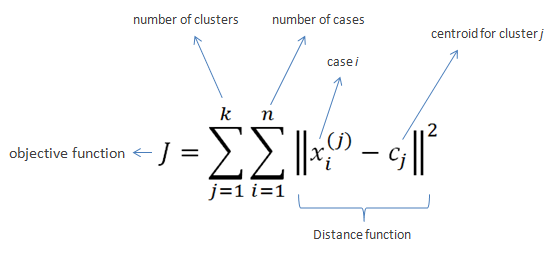
\includegraphics[width=0.5\textwidth]{img/ckmeans.png}
\end{figure}

 The algorithm as described by \cite{kmeans} starts with a random set of $k$ center-points ($\mu$). During each update step, all observations $x$ are assigned to their nearest center-point (see equation \ref{eqn:kmeans_assign_step}). In the standard algorithm, only one assignment to one center is possible. If multiple centers have the same distance to the observation, a random one would be chosen.

\begin{equation}
S_i^{(t)} = \big \{ x_p : \big \| x_p - \mu^{(t)}_i \big \|^2 \le \big \| x_p - \mu^{(t)}_j \big \|^2 \ \forall j, 1 \le j \le k \big\}
\label{eqn:kmeans_assign_step}
\end{equation}

Afterwards, the center-points are repositioned by calculating the mean of the assigned observations to the respective center-points (see \eqnref{kmeans_update_step}).

\begin{equation}
\mu^{(t+1)}_i = \frac{1}{|S^{(t)}_i|} \sum_{x_j \in S^{(t)}_i} x_j
\label{eqn:kmeans_update_step}
\end{equation}

The update process reoccurs until all observations remain at the assigned center-points and therefore the center-points would not be updated anymore.

% sample images

\begin{figure}
\centering
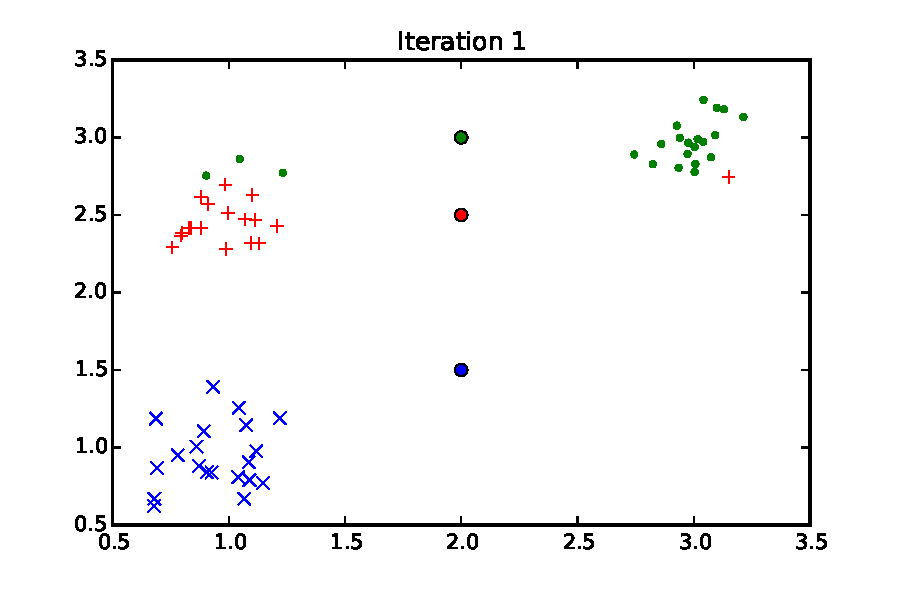
\includegraphics[width=0.4\linewidth]{img/iteration01}
\caption{k-Means: Possible initial centroid positions}
\label{fig:kmeans:iteration01}
\end{figure}

\begin{figure}
\centering
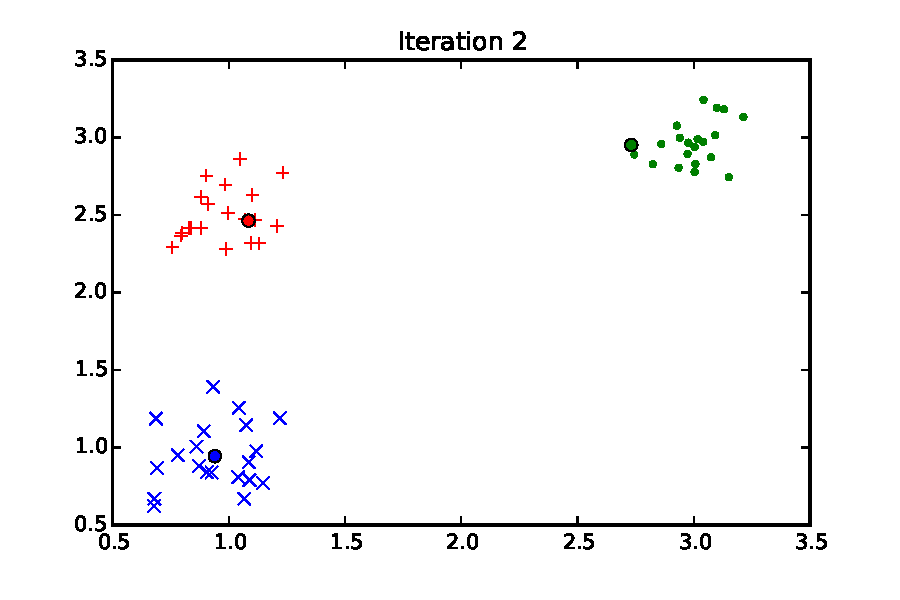
\includegraphics[width=0.4\linewidth]{img/iteration02}
\caption{k-Means: First iteration}
\label{fig:kmeans:iteration02}
\end{figure}

\begin{figure}
\centering
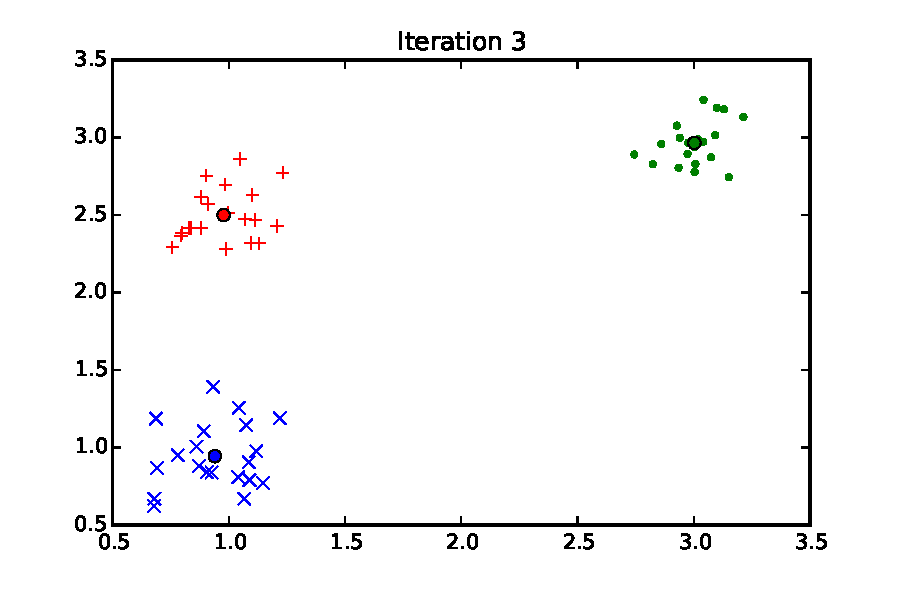
\includegraphics[width=0.4\linewidth]{img/iteration03}
\caption{k-Means: Second iteration}
\label{fig:kmeans:iteration03}
\end{figure}


This means that the k-means algorithm tries to optimize the objective function \ref{eqn:kmeans_objective_function}. As there is only a finite number of possible assignments for the amount of centroids and observations available and each iteration has to result in better solution, the algorithm always ends in a local minimum.

\begin{equation}
J = \sum_{n=1}^{N} \sum_{k=1}^{K} r_{nk} ||x_n - \mu_k||^2
\label{eqn:kmeans_objective_function}
\end{equation}

\[
\text{with } \\
r_{nk} = \begin{cases}
%1 & \text{if } k = \arg \min_j ||x_n - \mu_j||^2 \\
1 & x_n \in S_k \\
0 & \text{otherwise}
\end{cases}
\]

% minimize graph image

The main problem of k-means is its dependency on the initially chosen centroids. The centroids could end up in splitting common data points whilst other, separated points get grouped together if some of the centroids are more attracted by outliers. This points will get pulled to the same group of data points as shown in figure \ref{fig:kmeans_bad}.


\begin{figure}[h]
\centering
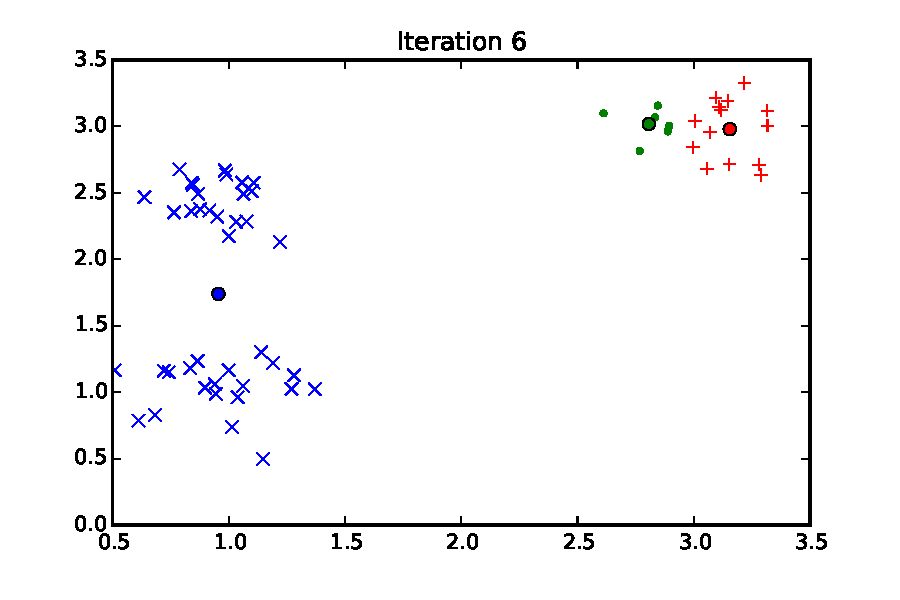
\includegraphics[width=0.4\linewidth]{img/kmeans_bad}
\caption{k-Means: Badly chosen initial center points}
\label{fig:kmeans_bad}
\end{figure}

The most common approach is to perform multiple clusterings with different start positions. Afterwards the clustering, which occurred most is considered as correct. Another, newer approach is the so called k-means++ by Arthur and Vassilvitskii \cite{Arthur}. This extension to the k-means algorithm tries to distribute the initial centroids over the given data to minimize the probability of bad outcomes. The initial points are set according to the authors by the following steps

\begin{enumerate}
    \item Take uniformly a random data point from the data $X$ and mark it as centroid $c_1$
    \item Choose another centroid $c_i$ with the probability $\frac{D(x)^2}{\sum_{x \in X} D(x)^2}$ where $D(x)$ denotes the shortest distance from the data point $x$ to its closest, already chosen centroid.
    \item Repeat 2. until all $k$ initial centroids are chosen.
\end{enumerate}
Afterwards, the standard k-means algorithm as described above is performed. The authors also showed that with this initialization algorithm, k-means++ approximately can be computed in $O(\log n)$, compared to $O(n^{dk+1} \log n)$ for the standard algorithm.



\section{Model Selection } \label{ms}
Model selection is the process of choosing between different machine learning approaches  or choosing between different hyperparameters or sets of features for the same machine learning approach  like in SVM kernels deciding between the polynomial degrees and  linear kernels .\\
The choice of the actual machine learning algorithm is less important than we'd think  there may be a "best" algorithm for a particular problem, but often its performance is not much better than other well performing approaches for that problem.

There may be certain qualities we look for in an model:

\begin{itemize}
\item Interpretable   can we see or understand why the model is making the decisions it makes?
\item Simple   easy to explain and understand
\item Accurate
\item Fast (to train and test)
\item Scalable (it can be applied to a large dataset)

\end{itemize}
Though there are generally trade offs among these qualities.\\in order to select a model from other models, we usually use one of the following approaches  .


\textbf{A Typical approach } is to take your data and split it randomly into a training set and a test set (e.g. a 70\%/30\% split). Then you train your model on the training set and see how it performs on the test set.

the problem with this Approach is it results in an overly optimistic estimation of generalization if we tune our model's parameters with it . so what we want to do instead is splitting the data is to not split it only into training and testing sets, but to also include a validation set. A typical ratio is 60\% training, 20\% validation, 20\% testing.

this way we can measure Validation error instead of just measuring the test error .

we can use these errors   to identify what kind of problem we have if our model isn't performing well:

\begin{itemize}
\item If our training error is large and our validation/test set error is large, then we have a high bias (underfitting) problem.
\item If our training error is small and our validation/test set error is large, then we have a high variance (overfitting) problem.
\end{itemize}

as the figure \ref{fig:bias} Explains : 

\begin{figure}[H]
\centering
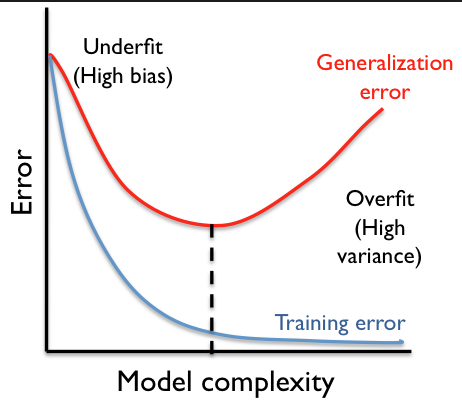
\includegraphics[width=0.5\textwidth]{img/model.png}
\caption{ bias / variance Tradeoff}
\label{fig:bias}
\end{figure}

Some ways of evaluating a model's performance on (some of)  known data are for \textbf{validation set } to pick  the best model you can possibly get :

\begin{itemize}
\item hold out (just set aside some portion of the data for validation; this is less reliable if the amount of data is small such that the held out portion is very small) 
\item k-fold cross-validation (better than hold out for small datasets) for better visualization  check figure \ref{fig:cross}
\begin{itemize}
\item the training set is divided into k folds
\item iteratively take k-1 folds for training and validate on the remaining fold
\item average the results
\item there is also "leave-one-out" cross-validation which is k-fold cross-validation where k=n (n is the number of data points)
\end{itemize}

\begin{figure}[H]
\centering
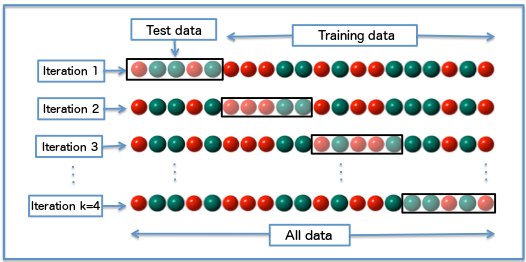
\includegraphics[width=1.0\textwidth]{img/cross.jpg}
\caption{K-cross validation }
\label{fig:cross}
\end{figure}


\item bootstrapping : 
\begin{itemize}
\item new datasets are generated by sampling with replacement (uniformly at random) from the original dataset
\item then train on the bootstrapped dataset and validate on the unselected data
\end{itemize}
\item jackknife resampling : 
essentially to leave-one-out cross-validation, since leave-one-out is basically sampling without replacement
\end{itemize}


\subsection{Evaluating classification models}\label{eva}

here is some important quantities we need to know in order to evaluate a model :
\begin{itemize}
\item Sensitivity: $ \frac{TP}{TP+FN}$ 
\item Specificity: $\frac{TN}{TN+FP}$
\item Positive predictive value:  $\frac{TP}{TP+FP}$ 
\item Negative predictive value: $\frac{TN}{TN+FN}$
\item Accuracy : $\frac{TP+TN}{TP+FP+TN+FN}$
\end{itemize}

\subsubsection{Area under the curve (AUC)}

This method is for binary classification and multilabel classification. In binary classification we may choose some cutoff above which we assign a sample to one class, and below which we assign a sample to the other class.Depending on our cutoff, we will get different results - there is a trade off between the true and false positive rates.\\
we can plot a Receiver Operating Characteristic (ROC) curve, which has for its y-axis \textbf{P(TP)}  and for its x-axis \textbf{P(FP)} . Every point on the curve corresponds to a cutoff value. That is, the ROC curve visualizes a sweep through all the cutoff thresholds so we can see the performance of our classifier across all cutoff thresholds, whereas other metrics (such as the F-score and so on) only tell we the performance for one particular cutoff. By looking at all thresholds at once, we get a more complete and honest picture of how our classifier is performing, in particular, how well it is separating the classes. It is insensitive to the bias of the data's classes  that is, if there are way more or way less of the positive class than there are of the negative class (other metrics may be deceptively favorable or punishing in such unbalanced circumstances).

The area under the curve (AUC) is used to quantify how good the classification algorithm is. In general, an AUC of above 0.8 is considered "good". An AUC of 0.5 (a straight line) is equivalent to random guessing.  


\begin{figure}[H]
\centering
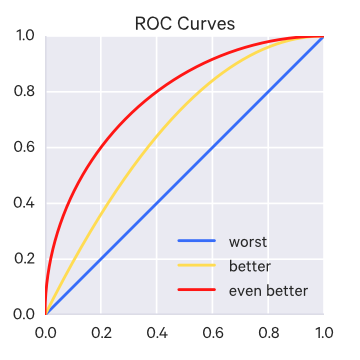
\includegraphics[width=0.5\textwidth]{img/roc.jpg}
\caption{ ROC curves }
\label{fig:bias2}
\end{figure}
So ROC curves (and the associated AUC metric) are very useful for evaluating binary classification.\\Note that ROC curves can be extended to classification of three or more classes by using the one-vs-all approach \\

\textbf{AUC incorporate the explanation below as well :}
AUC is a metric for binary classification and is especially useful when dealing with high-bias data, that is, where one class is much more common than the other. Using accuracy as a metric falls apart in high-bias datasets: for example, say ou have 100 training examples, one of which is is positive, the rest of which are negative. we could develop a model which just labels every thing negative, and it would have 99\% accuracy. So accuracy doesn't really tell  enough here.\\Many binary classifies output some continuous value (0-1), rather than class labels; there is some threshold (usually 0.5) above which one label is assigned, and below which the other label is assigned. Some models may work best with a different threshold. Changing this threshold leads to a trade off between true positives and false positives   for example, decreasing the threshold will yield more true positives, but also more false positives.\\AUC runs over all thresholds and plots the the true vs false positive rates. This curve is called a receiver operating characteristic curve, or ROC curve. A random classifier would give we equal false and true positives, which leads to a AUC of 0.5; the curve in this case would be a straight line. The better the classifier is, the more area under the curve there is (so the AUC approaches 1).

\subsubsection{Confusion Matrices}
This method is suitable for binary or multiclass classification.

For classification, evaluation often comes in the form of a confusion matrix.

The core values are:
\begin{itemize}
\item True positives (TP): samples classified as positive which were labeled positive
\item True negatives (TN): samples classified as negative which were labeled negative
\item False positives (FP): samples classified as positive which were labeled negative
\item False negatives (FN): samples classified as negative which were labeled positive\\

\textit{A few other metrics are computed from these values }:\\

\item Accuracy: How often is the classifier correct  $\frac{\text{TP} + \text{TN}}{\text{total}}$

\item Misclassification rate (or "error rate"): How often is the classifier wrong $\frac{\text{FP} + \text{FN}}{\text{total}} = 1 $-$ \text{accuracy}$

\item Recall (or "sensitivity" or "true positive rate"): How often are positive-labeled samples predicted as positive $\frac{\text{TP}}{\text{num positive-labeled examples}}$

\item False positive rate: How often are negative-labeled samples predicted as positive  $\frac{\text{FP}}{\text{num negative-labeled examples}}$

\item Specificity (or "true negative rate"): How often are negative-labeled samples predicted as negative  $\frac{\text{TN}}{\text{num negative-labeled examples}}$
\item Precision: How many of the predicted positive samples are correctly predicted   $\frac{\text{TP}}{\text{TP} + \text{FP}}$

\item Prevalence: How many labeled-positive samples are there in the data  $\frac{\text{num positive-labeled examples}}{\text{num examples}}$ 

Some other values:\\

\item Positive predictive value (PPV): precision but takes prevalence into account. With a perfectly balanced dataset (i.e. equal positive and negative examples, that is prevalence is 0.5), the PPV equals the precision.

\item F-score: The weighted average of recall and precision

\item ohen's Kappa: a measure of how well the classifier performs compared against if it had just guessed randomly, that is a high Kappa score happens when there is a big difference between the accuracy and the null error rate.

\end{itemize}

\subsection{Metric selection}
When it comes to skewed classes (or high bias data), metric selection is more nuanced.

For instance, say we have a dataset where only 0.5\% of the data is in category 1 and the rest is in category 0. we run our model and find that it categorized 99.5\% of the data correctly! But because of the skew in that data, our model could just be: classify each example in category 0, and it would achieve that accuracy.

Note that the convention is to set the rare class to 1 and the other class to 0. That is, we try to predict the rare class.

Instead, we may want to use \textbf{precision/recall} as our evaluation metric.

\begin{figure}[H]
\centering
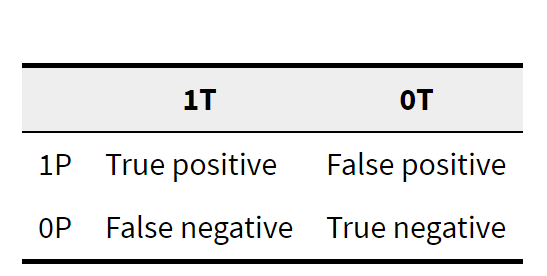
\includegraphics[width=0.6\textwidth]{img/TP.PNG}
\caption{  confusion matrix.}
\label{fig:TP}
\end{figure}

Where 1T/0T indicates the actual class and 1P/0P indicates the predicted class.\\
\textbf{Precision} is the number of true positives over the total number predicted as positive. That is, what fraction of the examples labeled as positive actually are positive  $\frac{\text{true positives}}{\text{true positives} + \text{false positives}}$ .\\
\textbf{Recall} is the number of true positives over the number of actual positives. That is, what fraction of the positive examples in the data were identified  $\frac{\text{true positives}}{\text{true positives} + \text{false negatives}}$


\section{Conclusion:}

in this chapter we have discussed in detail some of the most Popular classification algorithms in supervised  learning such As SVM ( Support vector machine ) , NN (Nearest neighbor ) and in  unsupervised learning the  k-means algorithm  , which are going to be used in the classification process after we fed them with the local descriptor such as Surf and Feature shape descriptor as of Fouriere coefficients ,  Next we studied different Methods for selecting $^{[\ref{ms}]}$ a Model Using K cross validation and bootstraping , and their astonishing role in maximization the performance of a classifier .
Finally we reviewed  how to  assess the performance of a fully trained classifier Using Area Under Curve ( AUC ) and Confusion matrix .

in the next chapter we will finally take a look on the techniques used in our HGR system  , and discussing multiple  project results.    


